\documentclass[11pt, a4paper]{article}

\usepackage{fontenc}
\usepackage{inputenc}
\usepackage{microtype}
\usepackage{amsmath, amssymb, amsthm}
\usepackage{geometry}
\usepackage{setspace}
\usepackage{titlesec}
\usepackage{hyperref}
\usepackage{fancyhdr}
\usepackage{abstract}
\usepackage{csquotes}
\usepackage{parskip}
\usepackage{mathtools}
\usepackage{enumitem}
\usepackage{tikz}
\usetikzlibrary{arrows.meta,calc,positioning,decorations.pathmorphing,shapes.geometric}

\geometry{
  top=1.25in,
  bottom=1.25in,
  left=1.375in,
  right=1.375in
}

\onehalfspacing

\hypersetup{
  colorlinks=true,
  linkcolor=black,
  citecolor=black,
  urlcolor=black,
  pdftitle={Trajectories All the Way Down: Movement as the Generative Principle of Geometry, Cognition, and Computation},
  pdfauthor={Flyxion}
}

\titleformat{\section}{\large\bfseries}{}{0em}{}[\titlerule]
\titleformat{\subsection}{\normalsize\bfseries\itshape}{}{0em}{}

\pagestyle{fancy}
\fancyhf{}
\rhead{\small\itshape Flyxion}
\lhead{\small\itshape Trajectories All the Way Down}
\cfoot{\thepage}
\renewcommand{\headrulewidth}{0.4pt}

\renewcommand{\abstractnamefont}{\normalfont\bfseries}
\renewcommand{\abstracttextfont}{\normalfont\small}

\theoremstyle{plain}
\newtheorem{theorem}{Theorem}[section]
\newtheorem{proposition}[theorem]{Proposition}
\newtheorem{corollary}[theorem]{Corollary}
\theoremstyle{definition}
\newtheorem{definition}[theorem]{Definition}
\theoremstyle{remark}
\newtheorem*{remark}{Remark}

\begin{document}

\begin{titlepage}
\centering
\vspace*{2cm}
{\LARGE\bfseries Trajectories All the Way Down}\\[0.8em]
{\large\itshape Movement as the Generative Principle of Geometry, Cognition, and Computation}\\[2.5cm]
{\large Flyxion}\\[0.5em]
{\normalsize Independent Scholar}\\[2cm]
{\normalsize\today}\\[3cm]
\begin{abstract}
\noindent This essay advances a single unifying claim: complex structures in mathematics,
neuroscience, cognition, and computation are not static objects stored in systems
but the outcomes of trajectories through spaces generated by simple transformations.
Scaling, rotation, and oscillation function as universal geometric primitives.
When composed into chains of operators, these primitives produce mathematical functions,
neural dynamics, semantic reasoning, and computational representations indistinguishable
in their underlying architecture. The essay traces this principle from classical sweep
geometry and complex analysis through Lie group theory, central pattern generators,
hippocampal navigation, information geometry, and deep learning, arguing that dimension,
thought, and meaning all arise from the same source: movement through representational
space. A philosophical consequence follows. Cognition does not store representations;
it generates them. Knowledge is not retrieved but traversed. The mind is less an archive
than a vehicle, and its objects less locations than roads.
\end{abstract}
\end{titlepage}

\newpage
\tableofcontents
\newpage


%%% ─────────────────────────────────────────────────────
\section{Introduction: Against the Static View of Structure}
%%% ─────────────────────────────────────────────────────

Modern science has inherited a tendency to treat the objects it studies as things that
exist rather than as processes that occur. A point in mathematics is defined by its
coordinates. A memory in neuroscience is assumed to reside somewhere in neural tissue.
A concept in cognitive psychology is imagined as a node in a network, a discrete element
connected to other discrete elements. A representation in machine learning is a vector
of real numbers frozen at a moment in computation. In each case, the dominant metaphor
is storage: knowledge, form, and meaning are housed in structures that persist, waiting
to be accessed.

This essay argues that the storage metaphor is systematically misleading. It produces
accurate descriptions at a surface level while obscuring the generative dynamics that
make structures possible in the first place. A triangle is not a set of three points;
it is the minimal network of traversable paths among three locations. A memory is not
a pattern inscribed in synaptic weights; it is a trajectory the brain can reliably
reconstruct through its own dynamics. A concept is not a node but a region in a
high-dimensional associative manifold, defined by the attractor geometry of the
cognitive system rather than by any fixed content.

The unifying thesis of this essay can be stated simply. Complex functions, concepts,
and behaviors emerge from compositions of simple transformations generated by
movement---scaling, rotation, and oscillation---applied to representational spaces.
What appears as structure in mathematics, perception, or semantic reasoning can therefore
be interpreted as trajectories produced by chained operators. The structure does not
precede the motion; it is the motion, stabilized and made readable.

\begin{figure}[h]
\centering
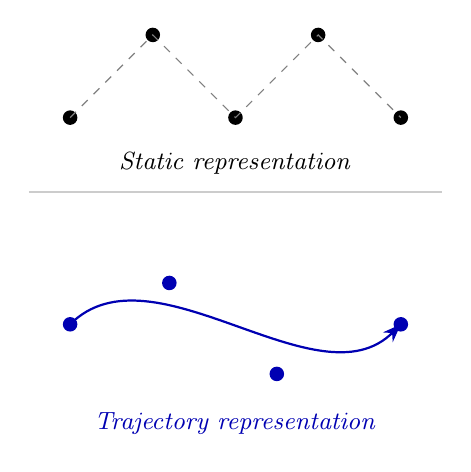
\begin{tikzpicture}[scale=1.05]
% Static nodes
\foreach \x/\y in {0/0,1/1,2/0,3/1,4/0}
    \fill (\x,\y) circle (2.5pt);
\draw[gray,dashed] (0,0)--(1,1)--(2,0)--(3,1)--(4,0);
\node at (2,-0.55) {\small\textit{Static representation}};

% Trajectory path
\draw[thick,blue!70!black,-{Stealth}]
  (0,-2.5) .. controls (1,-1.5) and (3,-3.5) .. (4,-2.5);
\foreach \x/\y in {0/-2.5, 1.2/-2.0, 2.5/-3.1, 4/-2.5}
    \fill[blue!70!black] (\x,\y) circle (2.5pt);
\node[blue!70!black] at (2,-3.7) {\small\textit{Trajectory representation}};

\draw[thick,gray!40] (-0.5,-.9) -- (4.5,-.9);
\end{tikzpicture}
\caption{Static node-based representations contrasted with trajectory-based
representations. The same points appear in both, but the trajectory view privileges
the paths that generate them.}
\end{figure}

This thesis is not merely metaphorical. It draws on a deep family of mathematical
results showing that rotation and scaling, as geometric primitives, generate universal
approximators when composed. It connects to empirical findings in systems neuroscience
showing that the same hippocampal circuits used for spatial navigation are reused for
conceptual reasoning. It aligns with the architecture of modern deep learning, where
stacked layers of simple linear and nonlinear operators approximate arbitrarily complex
functions. And it resonates with the philosophy of embodied cognition, which has long
argued that abstract reasoning is grounded in sensorimotor dynamics.

The essay develops this argument across fifteen sections. It begins with classical
geometry, where the generative role of motion in producing higher-dimensional objects
is already explicit. It then introduces Lie theory and the amplitwist interpretation of
complex differentiation. From there it moves through Fourier decomposition, biological
oscillators, spatial navigation, semantic cognition, control systems, image analysis,
information geometry, category theory, and the evolutionary origins of trajectory-based
cognition, showing that the same structural principle reappears at every level. The
essay also includes a section on empirical predictions, a mathematical appendix proving
the amplitwist decomposition, and a philosophical conclusion. If successful, the reader
should finish the essay unable to think of a line, a memory, or a neural activation
without also thinking of a path.


%%% ─────────────────────────────────────────────────────
\section{Sweep Geometry and the Generative Role of Motion}
%%% ─────────────────────────────────────────────────────

Classical Euclidean geometry presents its objects as if they were discovered rather
than constructed. A point is defined as that which has position but no magnitude.
A line is defined as that which has length but no breadth. These definitions are static.
They describe objects by what they are, not by how they come to be.

Yet a rival tradition runs continuously through the history of geometry, one that treats
shape as the outcome of movement. In this tradition, a line is what a point traces when
it moves. A surface is what a line traces when it moves in a direction not contained in
itself. A volume is what a surface traces when it moves in a direction not contained in
itself. Each higher-dimensional object is the swept trajectory of a lower-dimensional one
under a motion that adds a new independent direction to the system.

\begin{figure}[h]
\centering
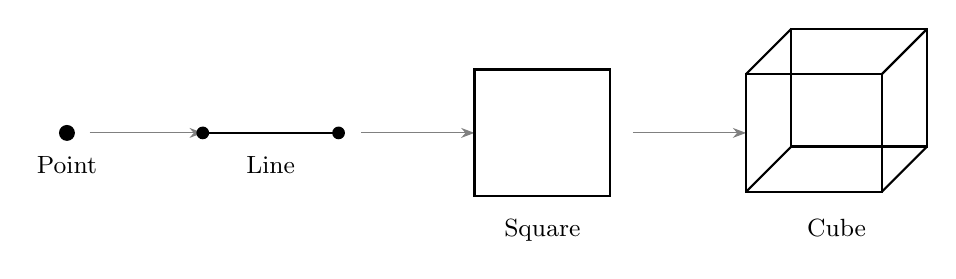
\begin{tikzpicture}[scale=1.15]
% Point
\fill (0,0) circle (2.5pt);
\node[below,font=\small] at (0,-0.15) {Point};

% Arrow to line
\draw[-{Stealth},gray] (0.25,0) -- (1.5,0);
\draw[thick] (1.5,0) -- (3,0);
\fill (1.5,0) circle (2pt); \fill (3,0) circle (2pt);
\node[below,font=\small] at (2.25,-0.15) {Line};

% Arrow to square
\draw[-{Stealth},gray] (3.25,0) -- (4.5,0);
\draw[thick] (4.5,-0.7) rectangle (6,0.7);
\node[below,font=\small] at (5.25,-0.85) {Square};

% Arrow to cube
\draw[-{Stealth},gray] (6.25,0) -- (7.5,0);
\draw[thick] (7.5,-0.65) rectangle (9,0.65);
\draw[thick] (8,-0.15) rectangle (9.5,1.15);
\draw[thick] (7.5,-0.65)--(8,-0.15);
\draw[thick] (9,-0.65)--(9.5,-0.15);
\draw[thick] (7.5,0.65)--(8,1.15);
\draw[thick] (9,0.65)--(9.5,1.15);
\node[below,font=\small] at (8.5,-0.85) {Cube};
\end{tikzpicture}
\caption{Higher-dimensional shapes as swept trajectories of lower-dimensional ones.
Each transition adds one new independent direction of motion.}
\end{figure}

This construction can be formalized with elementary parametric notation.
A line segment from point $\mathbf{a}$ to point $\mathbf{b}$ is the image of the map

\begin{equation}
\mathbf{x}(t) = (1-t)\mathbf{a} + t\mathbf{b}, \quad t \in [0,1].
\label{eq:line}
\end{equation}

As the parameter $t$ varies continuously from zero to one, a point moves along the
segment. The segment is not a collection of static points; it is the record of a motion.
Introducing a second independent parameter $s$ that translates the segment in a
direction perpendicular to $\mathbf{b} - \mathbf{a}$ produces a square. A third
independent parameter translates the square in a direction orthogonal to its plane and
produces a cube. In each case, the transition from one object to the next corresponds
not to an increase in the number of points stored but to the addition of a new
independent direction of motion.

A precise consequence follows from this perspective. Dimension is not an intrinsic
property of objects but a measure of the number of independent directions of motion
required to generate them. A curve is one-dimensional because it takes one parameter
to trace it. A surface is two-dimensional because it takes two independent parameters.
This interpretation shifts geometry from static description to generative dynamics.
The question is not what an object is but how it is produced.

The philosophical import of this shift is considerable. If dimension corresponds to
degrees of generative freedom, then mathematical objects encode motion rather than
merely extending through space. Geometry, understood in this way, is a science of
possible trajectories rather than a catalog of fixed forms.

The same logic applies in topology, where paths and homotopies---continuous deformations
of paths---are more fundamental than the spaces themselves in many contexts.
The fundamental group of a topological space is defined entirely in terms of based loops:
paths that begin and end at the same point. The space reveals its topology through the
structure of its possible motions, not through any intrinsic property of its points.
Sweep geometry, Lie theory, and homotopy theory all converge on the same intuition.
Structure is the record of transformation.


%%% ─────────────────────────────────────────────────────
\section{Lie Groups and the Algebra of Motion}
%%% ─────────────────────────────────────────────────────

The generative interpretation of geometry introduced in the previous section finds its
most systematic mathematical expression in Lie theory. Where sweep geometry emphasizes
the construction of objects from motion, Lie groups formalize the structure of the
motions themselves.

A Lie group is a smooth manifold whose elements represent transformations and whose
group operation corresponds to the composition of those transformations. Rotations of
three-dimensional space form the group $SO(3)$, translations form $\mathbb{R}^3$,
and rigid body motion combines both into the Euclidean group $SE(3)$.

The key insight of Lie theory is that global transformations can be generated from
infinitesimal ones. The tangent space at the identity element of a Lie group forms its
associated Lie algebra, whose elements act as generators of motion. Exponentiating
these generators produces finite transformations. For example, rotations about the
three coordinate axes generate all possible orientations of a rigid body:

\begin{equation}
R(\theta) = e^{\theta A},
\end{equation}

where $A$ is an element of the Lie algebra $\mathfrak{so}(3)$.
The exponential map carries infinitesimal twists into finite rotations.
The generators of the algebra are precisely the primitive directions of movement
in transformation space.

\begin{figure}[h]
\centering
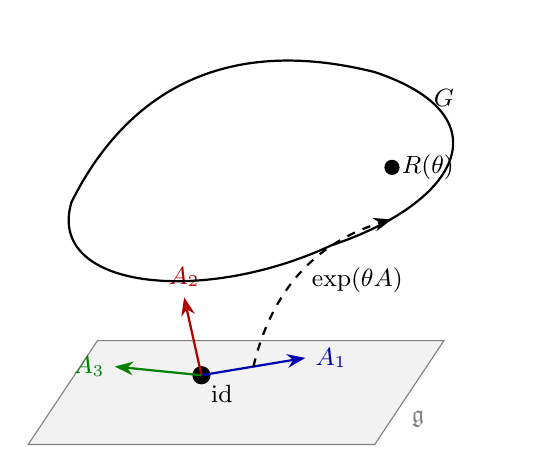
\begin{tikzpicture}[scale=1.1]
% Lie algebra tangent plane
\draw[fill=gray!10,draw=gray] (-2,-0.8) -- (2,-0.8) -- (2.8,0.4) -- (-1.2,0.4) -- cycle;
\node[gray] at (2.5,-0.5) {\small $\mathfrak{g}$};

% Identity point
\fill (0,0) circle (3pt);
\node[below right,font=\small] at (0,0) {$\mathrm{id}$};

% Algebra generator arrows
\draw[-{Stealth},blue!70!black,thick] (0,0) -- (1.2,0.2) node[right,font=\small]{$A_1$};
\draw[-{Stealth},red!70!black,thick] (0,0) -- (-0.2,0.9) node[above,font=\small]{$A_2$};
\draw[-{Stealth},green!50!black,thick] (0,0) -- (-1,0.1) node[left,font=\small]{$A_3$};

% Exponential arrow
\draw[-{Stealth},thick,dashed] (0.6,0.1) to[bend left=30] (2.2,1.8);
\node[font=\small] at (1.8,1.1) {$\exp(\theta A)$};

% Group manifold
\draw[thick] (1.5,1.5) .. controls (3,2) and (3.5,3) .. (2,3.5)
             .. controls (0,4) and (-1,3) .. (-1.5,2)
             .. controls (-1.8,1) and (0,0.8) .. (1.5,1.5);
\node at (2.8,3.2) {\small $G$};
\fill (2.2,2.4) circle (2.5pt);
\node[right,font=\small] at (2.2,2.4) {$R(\theta)$};
\end{tikzpicture}
\caption{The Lie algebra $\mathfrak{g}$ sits at the identity of the Lie group $G$
as a tangent space of generators. Exponentiating a generator $A$ produces a
one-parameter family of finite transformations on the group manifold.}
\end{figure}

From the perspective advanced in this essay, Lie algebras provide the mathematical
language for describing primitive motions. Each generator corresponds to a fundamental
direction of movement in transformation space. Complex structures arise from
exponentiating and composing these generators. This algebraic view of motion connects
directly to the amplitwist principle of the next section: rotation generators correspond
to twists in the local tangent space, while symmetric generators correspond to scaling
along principal axes. Together they span the transformation algebra that produces
structure through composition.

It is worth observing that many of the structures encountered in physics, geometry, and
machine learning carry implicit Lie group symmetries. The rotation group $SO(3)$ governs
the orientation of rigid bodies. The unitary group $U(n)$ governs the symmetries of
quantum states. The general linear group $GL(n)$ governs the full space of invertible
linear transformations applicable to neural representations. In each case, the group's
generators are the primitive directions through which the space of transformations is
navigated, and the exponential map converts those generators into traversable paths.
The abstract machinery of Lie theory is, in this sense, a precise formalization of the
essay's central intuition: global structure emerges from the composition of infinitesimal
motions.


%%% ─────────────────────────────────────────────────────
\section{The Amplitwist Principle: Complex Differentiation as Local Geometry}
%%% ─────────────────────────────────────────────────────

Complex analysis offers the most elegant instance of the essay's central thesis.
A function from the complex plane to itself is called holomorphic at a point if it is
complex-differentiable there. The geometric content of holomorphicity can be expressed
with disarming simplicity.

Consider a holomorphic function $f : \mathbb{C} \to \mathbb{C}$ that is differentiable
at a point $z_0$. In a sufficiently small neighborhood of $z_0$, the function behaves
approximately as

\begin{equation}
f(z_0 + \varepsilon) \approx f(z_0) + f'(z_0)\,\varepsilon.
\label{eq:amplitwist}
\end{equation}

The derivative $f'(z_0)$ is itself a complex number. Writing it in polar form,

\begin{equation}
f'(z_0) = \rho\,e^{i\theta},
\label{eq:polar}
\end{equation}

reveals its geometric content precisely. Multiplying the displacement $\varepsilon$
by $\rho$ scales it by the factor $\rho$. Multiplying by $e^{i\theta}$ rotates it by
the angle $\theta$. This is Needham's \emph{amplitwist}: an amplitude change and a twist
occurring simultaneously.

\begin{figure}[h]
\centering
\begin{tikzpicture}[scale=1.3]
\draw[-{Stealth},gray] (-2.2,0) -- (2.5,0) node[right]{\small Re};
\draw[-{Stealth},gray] (0,-1.8) -- (0,2.5) node[above]{\small Im};

% Original displacement
\draw[thick,-{Stealth}] (0,0) -- (1.4,0);
\node[below,font=\small] at (0.7,0) {$\varepsilon$};

% Rotated and scaled result
\draw[blue!70!black,thick,-{Stealth}] (0,0) -- (0.75,1.5);
\node[right,font=\small,blue!70!black] at (0.8,1.55) {$f'(z_0)\,\varepsilon$};

% Angle arc
\draw[-{Stealth},red!60!black] (0.9,0) arc (0:63:0.9);
\node[red!60!black,font=\small] at (1.1,0.5) {$\theta$};

% Rho label
\node[blue!60!black,font=\small] at (-0.35,0.75) {$\rho$};

\node[font=\small] at (0,-2.2) {rotation $\times$ scaling};
\end{tikzpicture}
\caption{Local amplitwist transformation in the complex plane. The derivative
$f'(z_0) = \rho e^{i\theta}$ simultaneously rotates $\varepsilon$ by angle $\theta$
and scales it by $\rho$.}
\end{figure}

The amplitwist interpretation has a direct consequence for the global behavior of
holomorphic functions. Because every holomorphic map acts locally as a rotation and
scaling, it is conformal: it preserves the angles between curves meeting at a point.
The global analytic structure of a holomorphic function emerges from the continuous
variation of these local amplitwist operations across the domain.

This establishes a mathematical prototype for the essay's central thesis. Complex,
globally-structured analytic mappings are built from chains of simple geometric
operations: local rotations and scalings that vary smoothly from point to point.
The complication of the global map arises not from any single large transformation but
from the accumulated composition of many small ones. Structure is the record of
trajectories through operator space.

The deeper significance of the amplitwist principle becomes apparent when one considers
conformal mappings and Riemann's mapping theorem. The theorem states that any simply
connected proper open subset of the complex plane is conformally equivalent to the open
unit disk. Such maps can be extremely complicated in explicit form, yet all of them can
be analyzed as compositions of local amplitwists. The Möbius transformations, which
form the group of conformal automorphisms of the Riemann sphere, are the simplest such
maps; they are generated by translations, scalings, rotations, and inversion, each of
which is an elementary geometric transformation. More complicated conformal mappings
are built from compositions of these generators.

The amplitwist decomposition---$f'(z_0) = \rho e^{i\theta}$---is also the content of
the polar decomposition theorem for linear transformations. Any invertible complex
linear map can be written as the product of a rotation and a positive scaling.
The amplitwist is therefore not a special property of complex numbers but a universal
decomposition available for any linear transformation. This universality will become
important in the sections on image analysis and latent representations.


%%% ─────────────────────────────────────────────────────
\section{Oscillatory Primitives and Universal Approximation}
%%% ─────────────────────────────────────────────────────

The amplitwist principle identifies rotation and scaling as the generators of complex
analytic structure. A parallel story unfolds in signal processing and computational
mathematics, where the generative role of oscillatory components is made explicit
through Fourier analysis.

The central result of classical Fourier theory is that any sufficiently well-behaved
periodic function can be expressed as a superposition of sinusoidal components:

\begin{equation}
f(x) = \sum_{n=-\infty}^{\infty} c_n\, e^{inx}.
\label{eq:fourier}
\end{equation}

Each term $e^{inx}$ is a pure oscillation, a rotation in the complex plane at angular
frequency $n$. The coefficient $c_n$ controls the amplitude. Complex signals arise from
compositions of simple oscillatory primitives.

\begin{figure}[h]
\centering
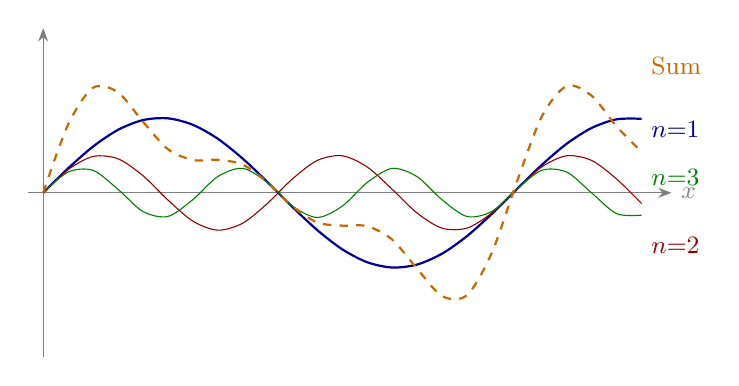
\begin{tikzpicture}[scale=0.95]
\draw[-{Stealth},gray] (-0.2,0) -- (8.4,0) node[right]{\small$x$};
\draw[-{Stealth},gray] (0,-2.2) -- (0,2.2);
\draw[domain=0:8,smooth,blue!60!black,thick] plot (\x,{sin(\x r)});
\draw[domain=0:8,smooth,red!60!black] plot (\x,{0.5*sin(2*\x r)});
\draw[domain=0:8,smooth,green!50!black] plot (\x,{0.33*sin(3*\x r)});
\draw[domain=0:8,smooth,thick,orange!80!black,dashed]
    plot (\x,{sin(\x r)+0.5*sin(2*\x r)+0.33*sin(3*\x r)});
\node[right,blue!60!black,font=\small] at (8,0.85) {$n{=}1$};
\node[right,red!60!black,font=\small] at (8,-0.7) {$n{=}2$};
\node[right,green!50!black,font=\small] at (8,0.2) {$n{=}3$};
\node[right,orange!80!black,font=\small] at (8,1.7) {Sum};
\end{tikzpicture}
\caption{A complex signal (dashed) arising from superposition of three oscillatory
primitives at frequencies $n=1,2,3$. Each component is a rotation in the complex plane
at the corresponding angular rate.}
\end{figure}

What does a single layer of a neural network do, geometrically? It applies a linear
transformation $W$ to an input vector $\mathbf{x}$, shifts the result by a bias
$\mathbf{b}$, and then applies a pointwise nonlinear function $\sigma$:

\begin{equation}
\mathbf{h} = \sigma(W\mathbf{x} + \mathbf{b}).
\label{eq:neuron}
\end{equation}

By the polar decomposition, the linear transformation $W$ can be analyzed as a rotation
followed by a scaling in each principal direction. The nonlinearity $\sigma$ then folds
and warps the resulting configuration, creating new curvature in the feature space.
Stacking many such layers composes many small geometric transformations until the
cumulative effect approximates a complicated mapping.

This architecture is the computational analogue of the amplitwist cascade. Just as a
complex analytic function is locally a rotation and scaling at every point, and its
global behavior emerges from composing these local operations, a deep neural network
computes a complex input-output mapping by composing many layers of small geometric
transformations. The universality of the approximation corresponds to the completeness
of the Fourier expansion: given enough layers and units, the chain of operators can
approximate any target function.


%%% ─────────────────────────────────────────────────────
\section{Central Pattern Generators and Phase-Space Geometry}
%%% ─────────────────────────────────────────────────────

The previous sections established that composition of geometric primitives produces
universal approximators in mathematics and computation. The same principle appears in
biological motor systems, but now the primitives are physically implemented by networks
of coupled oscillators.

Central pattern generators are neural circuits that produce rhythmic, patterned motor
output without requiring continuous sensory input. Their dynamics have been extensively
studied through coupled-oscillator models in which each unit contributes a simple
periodic rhythm and interactions among units produce coordinated patterns.

A single oscillator in a CPG circuit can be modeled as a two-dimensional dynamical
system with a stable limit cycle. If its state is represented as $z(t) = x(t) + iy(t)$,
its evolution corresponds to circular motion in the complex plane---a rotation at a fixed
radius, with amplitude modulated by coupling to other units.

\begin{figure}[h]
\centering
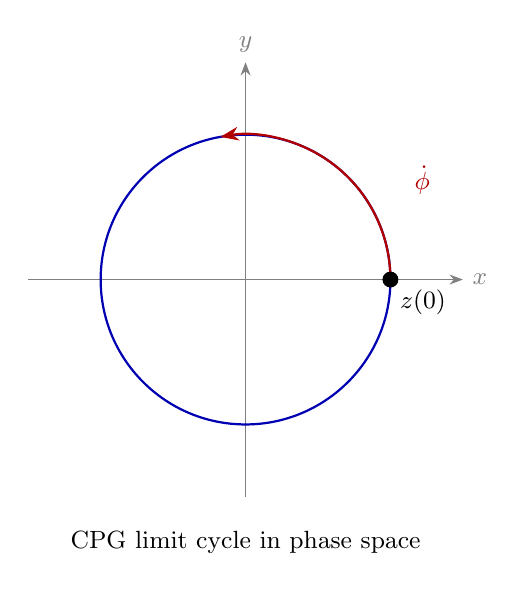
\begin{tikzpicture}[scale=1.15]
\draw[-{Stealth},gray] (-2.4,0) -- (2.4,0) node[right]{\small$x$};
\draw[-{Stealth},gray] (0,-2.4) -- (0,2.4) node[above]{\small$y$};

% Limit cycle
\draw[thick,blue!70!black] (0,0) circle (1.6);

% Phase arrow
\draw[red!70!black,thick,-{Stealth}] (1.6,0) arc (0:100:1.6);
\node[red!70!black,font=\small] at (1.95,1.1) {$\dot\phi$};

% Label
\fill (1.6,0) circle (2.5pt);
\node[below right,font=\small] at (1.6,0) {$z(0)$};
\node[font=\small] at (0,-2.9) {CPG limit cycle in phase space};
\end{tikzpicture}
\caption{A CPG oscillator traces a stable limit cycle in the complex phase plane.
Amplitude modulation scales the radius; phase coupling rotates the state along the cycle.
Together they implement the two components of an amplitwist.}
\end{figure}

When two or more such oscillators are coupled, their phase relationships evolve
according to coupling dynamics, canonically described by the Kuramoto model.
In a network of $N$ coupled oscillators with natural frequencies $\omega_i$,
the phase $\phi_i$ evolves as

\begin{equation}
\dot{\phi}_i = \omega_i + \frac{K}{N}\sum_{j=1}^{N}\sin(\phi_j - \phi_i),
\label{eq:kuramoto}
\end{equation}

where $K$ is the coupling strength. When $K$ exceeds a critical threshold, the
oscillators synchronize. Partial synchrony at intermediate coupling strengths produces
a rich variety of phase-locking patterns, each encoding a different spatial or temporal
structure in the motor output.

A CPG network is therefore a physical implementation of amplitwist cascades. Each
oscillator contributes a rotation in its local phase plane; coupling translates phase
information across the network. The motor pattern that emerges corresponds to a
trajectory in the high-dimensional phase space of the full network---stable, reproducible,
and parameterized by coupling strengths and intrinsic frequencies.

An animal that varies its gait from walking to trotting to galloping does not switch to
a completely different neural circuit; it modulates the coupling strengths and phase
offsets of the same oscillator network, moving from one stable trajectory to another.
The transitions between gaits correspond to bifurcations in the coupled-oscillator
dynamics. The body's movement repertoire is a collection of stable trajectories in CPG
phase space, navigated through the same control parameters that generate the individual
oscillations.

Neuromodulatory signals---dopamine, serotonin, norepinephrine---adjust the excitability
of CPG neurons, effectively changing the gain of the oscillation and scaling the
amplitude of the output rhythm. Phase coupling combined with neuromodulatory gain
control implements, at the biological circuit level, the precise operations identified
in complex analysis as the generators of conformal transformations.


%%% ─────────────────────────────────────────────────────
\section{Hippocampal Navigation and the Geometry of Cognitive Maps}
%%% ─────────────────────────────────────────────────────

The hippocampal formation provides the most empirically detailed example of a biological
system that generates structure through trajectories rather than storage. Place cells in
the hippocampus proper fire selectively when an animal occupies a specific region of its
environment. Grid cells in the medial entorhinal cortex fire at the vertices of a
regular hexagonal lattice that tiles the environment.

\begin{figure}[h]
\centering
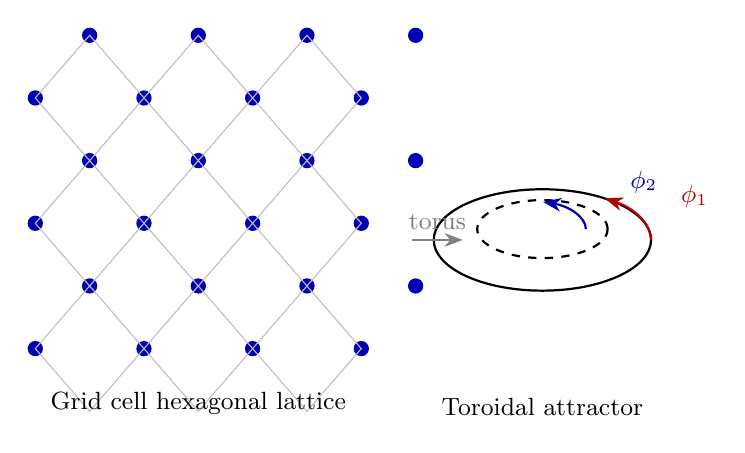
\begin{tikzpicture}[scale=0.92]
% Hexagonal grid
\foreach \x in {0,1.5,3,4.5}
{
  \foreach \y in {0,1.73,3.46}
  {
    \fill[blue!70!black] (\x,\y) circle (3pt);
    \fill[blue!70!black] (\x+0.75,\y+0.865) circle (3pt);
  }
}
% Hex lines
\foreach \x in {0,1.5,3}
  \draw[gray!50] (\x,0)--(\x+0.75,0.865)--(\x+1.5,0)--(\x+0.75,-0.865)--cycle;
\foreach \x in {0,1.5,3}
  \foreach \y in {1.73,3.46}
    \draw[gray!50] (\x,\y)--(\x+0.75,\y+0.865)--(\x+1.5,\y)--(\x+0.75,\y-0.865)--cycle;

\node[font=\small] at (2.25,-0.75) {Grid cell hexagonal lattice};

% Torus (right side)
\begin{scope}[xshift=7cm,yshift=1.5cm]
\draw[thick] (0,0) ellipse (1.5 and 0.7);
\draw[thick,dashed] (0,0.15) ellipse (0.9 and 0.4);
\draw[-{Stealth},red!70!black,thick] (1.5,0) arc (0:55:1.5 and 0.7);
\draw[-{Stealth},blue!70!black,thick] (0.6,0.15) arc (0:70:0.9 and 0.4);
\node[font=\small,red!70!black] at (2.1,0.6) {$\phi_1$};
\node[font=\small,blue!70!black] at (1.4,0.8) {$\phi_2$};
\end{scope}
\draw[-{Stealth},thick,gray] (5.2,1.5) -- (5.9,1.5) node[midway,above,font=\small]{torus};
\node[font=\small] at (7,-0.8) {Toroidal attractor};
\end{tikzpicture}
\caption{Left: Grid cell hexagonal lattice tiling an environment.
Right: The corresponding toroidal attractor structure. Grid codes correspond
mathematically to periodic coordinates on a torus, with two independent phase
variables $\phi_1$, $\phi_2$.}
\end{figure}

The mathematical relationship between grid cells and place cells can be understood as a
transformation between different coordinate representations of the same space. Grid cells
provide a Fourier-like basis for spatial location: the hexagonal periodicity at multiple
spatial scales and orientations constitutes a set of oscillatory components in
two-dimensional space. Place fields can be constructed by summing the activity of grid
cells at appropriate phases and scales, in a manner formally analogous to the synthesis
of a spatial pattern from frequency components.

Path integration is the mechanism by which the grid and place cell system maintains a
continuous estimate of position through movement. As the animal moves, velocity signals
are integrated over time to update the phase of each grid cell oscillator, moving the
animal's represented position through the cognitive map. The map is not retrieved from
storage but continuously reconstructed from movement.

The extension of this spatial navigation machinery to non-spatial cognition is one of
the most significant recent developments in cognitive neuroscience. Experiments using
functional neuroimaging have shown that grid-cell-like signals appear in the entorhinal
cortex when human subjects navigate abstract spaces. When participants learned
relationships among objects arranged in a two-dimensional conceptual grid defined by
abstract features, entorhinal activity exhibited the hexagonal periodicity characteristic
of spatial grid cells. The same neural machinery computed both spatial and conceptual
coordinates.

Andrea Hiott has developed a complementary account in recent work, arguing that the
neural machinery of spatial navigation constitutes a scaffold for the formation of
semantic memory. Her proposal is that \emph{way-making}---the activity of establishing
paths through an environment---underlies both physical navigation and cognitive processes
such as remembering, planning, and conceptual reasoning. In this view, the hippocampus
is not a memory storage device but a way-making engine: it generates trajectories through
structured spaces, whether those spaces are geographical or conceptual in character.
Representations, on this account, are communicative assessments of regularities in
embodied action---the ways in which the system has learned to move through its world.


%%% ─────────────────────────────────────────────────────
\section{Semantic Cognition as Navigation Through Attractor Landscapes}
%%% ─────────────────────────────────────────────────────

The static view of semantic memory treats concepts as nodes in a network, connected by
labeled edges encoding semantic relationships. A more geometrically explicit alternative
draws on the theory of conceptual spaces developed by Gärdenfors. In this framework,
concepts correspond to convex regions in a high-dimensional quality space, where
dimensions correspond to perceptual or functional properties.

The attractor-landscape model extends this framework by adding dynamics. In a
sufficiently rich associative system, activating one concept creates a gradient of
activation that spreads to nearby regions of the conceptual manifold, preferentially
activating concepts sharing contextual, co-occurrence, or causal structure with the
initial concept. This spreading activation defines attractor basins: regions of the
manifold toward which nearby trajectories converge. A schema---a structured scenario
such as RESTAURANT, HOSPITAL, or ARGUMENT---corresponds to a basin in this landscape,
where many conceptually related items cluster under a common contextual geometry.

\begin{figure}[h]
\centering
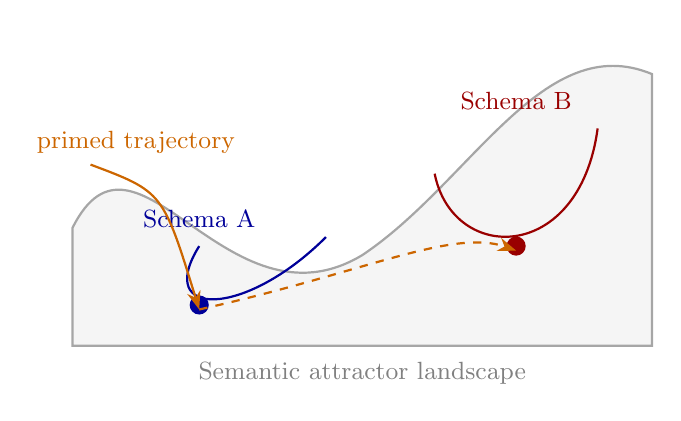
\begin{tikzpicture}[scale=1.15]
% Landscape surface approximation
\draw[thick,gray!70,fill=gray!8]
  (-3.2,-0.2) .. controls (-2.5,1.2) and (-1.5,-1.4) ..
  (0,-0.5) .. controls (1.2,0.3) and (2,2) ..
  (3.2,1.5) -- (3.2,-1.5) -- (-3.2,-1.5) -- cycle;

% Basin A
\draw[blue!60!black,thick] (-1.8,-0.4) .. controls (-2.3,-1.2) and (-1.3,-1.2) .. (-0.4,-0.3);
\fill[blue!60!black] (-1.8,-1.05) circle (3pt);
\node[blue!60!black,font=\small,above] at (-1.8,-0.3) {Schema A};

% Basin B
\draw[red!60!black,thick] (0.8,0.4) .. controls (1.0,-0.6) and (2.4,-0.6) .. (2.6,0.9);
\fill[red!60!black] (1.7,-0.4) circle (3pt);
\node[red!60!black,font=\small,above] at (1.7,1) {Schema B};

% Trajectory
\draw[-{Stealth},thick,orange!80!black]
  (-3,0.5) .. controls (-2.2,0.2) .. (-1.8,-1.1);
\draw[-{Stealth},thick,orange!80!black,dashed]
  (-1.8,-1.1) .. controls (0,-0.7) and (1,-0.2) .. (1.7,-0.45);
\node[orange!80!black,font=\small] at (-2.5,0.75) {primed trajectory};

\node[font=\small,gray] at (0,-1.8) {Semantic attractor landscape};
\end{tikzpicture}
\caption{Concepts as attractor basins in a semantic landscape. A priming stimulus
shifts the trajectory toward Schema A; subsequent associations can lead the trajectory
into Schema B. Reasoning follows gradient descent through the landscape, not
retrieval from storage.}
\end{figure}

Semantic priming can be understood in these terms as the perturbation of the cognitive
system's position in conceptual space. When a prime word is presented, it shifts the
system's representational state toward the region associated with that word, making
trajectories into nearby attractor basins more probable. The concept reached after
priming is not retrieved; it is arrived at through a shortened trajectory facilitated
by the initial perturbation.

Navigation through this landscape exhibits properties that distinguish it from symbolic
retrieval. Trajectories have duration: they take time to traverse attractor basins and
to transition between them. They have inertia: the system tends to continue in the
direction of current activation rather than jumping discontinuously to arbitrary
locations. They are sensitive to context: the same starting point can lead to different
destinations depending on the current gradient of activation across the manifold.
These are the hallmarks of dynamical navigation, not database lookup.

The amplitwist operators identified in previous sections provide the local transformation
primitives that deform and navigate this terrain: rotations in representational space
shift the alignment of concepts relative to one another, scalings modulate the relative
salience of different conceptual dimensions, and oscillatory dynamics provide the carrier
for maintaining coherent trajectories over time. A schema is not a template superimposed
on incoming information but an attractor basin whose geometry shapes the trajectories
of activation that pass through it. Inference is navigation: following the gradient of
the schema basin to its expected terminus.


%%% ─────────────────────────────────────────────────────
\section{Control Parameters and Degrees of Freedom in Transformation Space}
%%% ─────────────────────────────────────────────────────

The mathematical structure of a navigation system, whether physical or cognitive, can
be understood through the concept of degrees of freedom. A degree of freedom is an
independent parameter whose variation produces a distinct mode of change in the system's
state. A rigid body moving freely in three-dimensional physical space has six degrees of
freedom: three translational parameters specifying position and three rotational
parameters specifying orientation.

\begin{figure}[h]
\centering
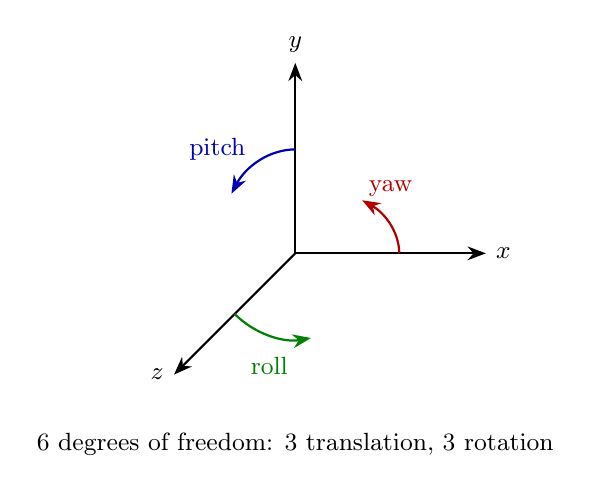
\begin{tikzpicture}[scale=1.1]
% Axes
\draw[-{Stealth},thick] (0,0,0) -- (2.2,0,0) node[right]{\small$x$};
\draw[-{Stealth},thick] (0,0,0) -- (0,2.2,0) node[above]{\small$y$};
\draw[-{Stealth},thick] (0,0,0) -- (-1.4,-1.4,0) node[left]{\small$z$};

% Rotation arcs
\draw[-{Stealth},red!70!black,thick] (1.2,0) arc (0:50:1.2 and 0.8);
\node[red!70!black,font=\small] at (1.1,0.75) {yaw};

\draw[-{Stealth},blue!70!black,thick] (0,1.2) arc (90:145:0.9 and 1.2);
\node[blue!70!black,font=\small] at (-0.9,1.2) {pitch};

\draw[-{Stealth},green!50!black,thick] (-0.7,-0.7) arc (225:280:1.0);
\node[green!50!black,font=\small] at (-0.3,-1.3) {roll};

\node[font=\small] at (0,-2.2) {6 degrees of freedom: 3 translation, 3 rotation};
\end{tikzpicture}
\caption{Degrees of freedom in a rigid body navigation system. Three translational and
three rotational generators span the full Euclidean group $SE(3)$. Any reachable
configuration is reached by composing motion along these axes.}
\end{figure}

The video game Descent provides an unusually pure illustration of this structure. Unlike
most navigation games restricted by gravitational constraints, Descent places the
player's vehicle in a fully three-dimensional microgravity environment where all six
degrees of freedom are simultaneously available. Navigation consists of continuously
adjusting these six control parameters, composing small local transformations to produce
complex global trajectories. The player does not compute a path; they navigate by
applying simple local controls that accumulate into whatever trajectory the task requires.

The analogy to the amplitwist framework is precise. In complex analysis, the generating
operations---rotation and scaling---provide two degrees of freedom at each point of the
domain. A conformal mapping is navigated through the continuous adjustment of these two
parameters. The global mapping emerges from the accumulated composition of local
adjustments, just as a global trajectory through three-dimensional space emerges from
the accumulated composition of local thrust and rotation commands.

The space of all transformations of a given type is itself a geometric space, often a
Lie group. A point in transformation space represents a specific transformation. Moving
through transformation space corresponds to composing transformations in a continuous
way. The generating operations of the transformation group---the Lie algebra
generators---play the role of control axes: they are the minimal set of infinitesimal
motions from which all transformations in the group can be reached.


%%% ─────────────────────────────────────────────────────
\section{Image Analysis and the Latent Geometry of Representations}
%%% ─────────────────────────────────────────────────────

An image can be formally represented as a vector $\mathbf{x} \in \mathbb{R}^n$,
where $n$ is the total number of pixel values. The images that arise from natural
scenes occupy a small, structured subset of this space: a manifold of much lower
intrinsic dimension, curved through the ambient space in a way that reflects
the statistical regularities of natural image structure.

A geometric transformation applied to an image corresponds to movement along a specific
direction in this manifold. The basic linear transformation can be written as

\begin{equation}
\mathbf{y} = A\mathbf{x},
\label{eq:linear_transform}
\end{equation}

where $A$ is a transformation matrix. By the polar decomposition theorem, $A = RS$,
where $R$ is orthogonal and $S$ is symmetric positive definite. An orthogonal
transformation preserves all distances and angles; the image is reoriented without being
distorted. The symmetric factor stretches or compresses the image along its principal
axes. Every linear image transformation is, therefore, an amplitwist: a composition of
rotation and scaling.

\begin{figure}[h]
\centering
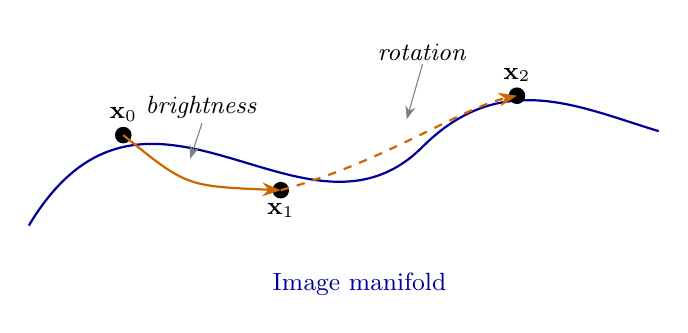
\begin{tikzpicture}[scale=1.0]
% Image manifold curve
\draw[thick,blue!60!black]
  (0,0) .. controls (1.5,2.5) and (3.5,-.5) .. (5,1)
        .. controls (6,2) and (7,1.5) .. (8,1.2);
\node[blue!60!black,font=\small] at (4.2,-0.75) {Image manifold};

% Points on manifold
\fill (1.2,1.15) circle (3pt); \node[above,font=\small] at (1.2,1.2) {$\mathbf{x}_0$};
\fill (3.2,0.45) circle (3pt); \node[below,font=\small] at (3.2,0.4) {$\mathbf{x}_1$};
\fill (6.2,1.65) circle (3pt); \node[above,font=\small] at (6.2,1.7) {$\mathbf{x}_2$};

% Trajectory arrows
\draw[-{Stealth},orange!80!black,thick]
  (1.2,1.15) .. controls (2,0.5) .. (3.2,0.45);
\draw[-{Stealth},orange!80!black,thick,dashed]
  (3.2,0.45) .. controls (4.5,0.8) and (5.5,1.5) .. (6.2,1.65);

% Slider annotation
\node[font=\small] at (2.2,1.5) {\textit{brightness}};
\draw[-{Stealth},gray,thin] (2.2,1.3) -- (2.05,0.85);
\node[font=\small] at (5,2.2) {\textit{rotation}};
\draw[-{Stealth},gray,thin] (5,2.05) -- (4.8,1.35);
\end{tikzpicture}
\caption{Images as points on a curved manifold in high-dimensional space.
Adjustable parameters (brightness, rotation) correspond to navigable directions
along the manifold. Each slider is literally a coordinate in transformation space.}
\end{figure}

In practical image editing, this structure manifests as the set of available adjustment
controls. Brightness, contrast, gamma, exposure, hue, saturation, and sharpness each
correspond to a specific combination of linear and nonlinear transformations in the image
representation space. The slider for each control moves the image along a specific
direction in that space. Adjusting multiple controls simultaneously navigates a
multi-dimensional subspace, tracing a trajectory through the image manifold parameterized
by the control values.

In latent representations learned by autoencoders or diffusion models, directions in
latent space correspond to interpretable image transformations: pose change, lighting
variation, identity in a face recognition system. Moving along these directions produces
smooth, semantically meaningful variations in the reconstructed image. In diffusion
models, the generation of a new image from noise is literally a trajectory: a path
through image space guided by a learned vector field at each point. The composition of
many small denoising steps accumulates into a coherent image through the same principle
of generating complex structure from chained simple operators that runs through this
entire essay.


%%% ─────────────────────────────────────────────────────
\section{Information Geometry and Statistical Manifolds}
%%% ─────────────────────────────────────────────────────

The trajectory view of cognition and computation acquires additional mathematical
clarity through information geometry, a field that studies statistical models as
geometric manifolds. In information geometry, a probability distribution $p(x|\theta)$
is treated as a point on a manifold whose coordinates are the parameters $\theta$.
Distances between distributions are measured using the Fisher information metric,

\begin{equation}
g_{ij}(\theta) =
\mathbb{E}\left[
\frac{\partial \log p(x|\theta)}{\partial \theta_i}
\frac{\partial \log p(x|\theta)}{\partial \theta_j}
\right].
\label{eq:fisher}
\end{equation}

\begin{figure}[h]
\centering
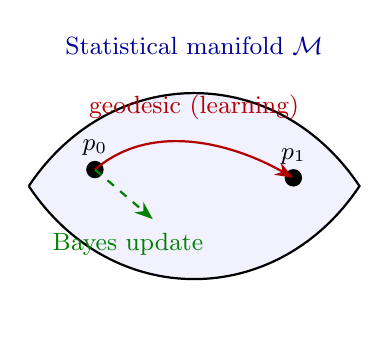
\begin{tikzpicture}[scale=1.05]
% Statistical manifold
\draw[thick,fill=blue!5]
  (0,0) .. controls (1,1.5) and (3,1.5) .. (4,0)
        .. controls (3,-1.5) and (1,-1.5) .. (0,0);

\node[font=\small,blue!60!black] at (2,1.7) {Statistical manifold $\mathcal{M}$};

% Points
\fill (0.8,0.2) circle (3pt); \node[above,font=\small] at (0.8,0.25) {$p_0$};
\fill (3.2,0.1) circle (3pt); \node[above,font=\small] at (3.2,0.15) {$p_1$};

% Geodesic
\draw[-{Stealth},red!70!black,thick]
  (0.8,0.2) .. controls (1.5,0.8) and (2.5,0.5) .. (3.2,0.1);
\node[red!70!black,font=\small] at (2,0.95) {geodesic (learning)};

% Bayesian update arrow
\draw[-{Stealth},green!50!black,thick,dashed] (0.8,0.2) -- (1.5,-0.4);
\node[green!50!black,font=\small] at (1.2,-0.7) {Bayes update};
\end{tikzpicture}
\caption{The statistical manifold of probability distributions parameterized by
$\theta$, equipped with the Fisher information metric. Learning corresponds to
geodesic paths; Bayesian updating moves the distribution along shorter locally
curved paths determined by the metric geometry.}
\end{figure}

Learning and inference correspond to trajectories on this manifold. Gradient descent
follows the steepest path toward a minimum of the loss function, while Bayesian updating
moves the system along geodesics determined by new data. The training of a neural network
is literally navigation through a statistical manifold. Each update step is a local
movement in parameter space guided by the geometry of the Fisher metric. Natural gradient
methods---which replace the Euclidean gradient with the Fisher-metric gradient---make
this geometric interpretation operationally precise: they follow the geodesic path of
steepest descent on the information manifold rather than in raw parameter space.

The connection to the trajectory framework developed in this essay is direct. Just as
spatial navigation traces paths through physical environments, statistical learning
traces paths through information space. The operators applied during learning are
geometric transformations that reshape the representation manifold until trajectories
converge on stable attractors corresponding to learned solutions. The Fisher metric
governs the local geometry, playing a role analogous to the Riemannian metric on the
cognitive manifolds described in earlier sections.

Seen in this light, overfitting corresponds to a trajectory that descends too aggressively
into a narrow well of the loss landscape without finding a broad, stable attractor.
Regularization corresponds to the imposition of geometric constraints on the allowable
trajectories, analogous to the entropy field $S$ in the RSVP framework that prevents
runaway amplification. In both biological and artificial learning systems, the geometry
of the learning trajectory shapes what can be generalized and what cannot.


%%% ─────────────────────────────────────────────────────
\section{Toward a Unified Geometric Model}
%%% ─────────────────────────────────────────────────────

The preceding sections have traced the essay's central thesis through ten distinct
domains. It is now possible to state their convergence as a unified geometric model
of cognition and computation.

Let $\mathcal{M}$ be a smooth manifold representing the state space of some system.
A \emph{representational state} of the system is a point $p \in \mathcal{M}$.
A \emph{primitive operator} is a smooth map $T : \mathcal{M} \to \mathcal{M}$ that
implements a local rotation, scaling, or oscillatory phase shift in the tangent space
at each point. A \emph{trajectory} is a smooth curve $\gamma : [0,1] \to \mathcal{M}$
produced by the continuous application of a sequence of primitive operators.
A \emph{structure} is a trajectory or family of related trajectories that the system
reliably produces under given conditions.

\begin{figure}[h]
\centering
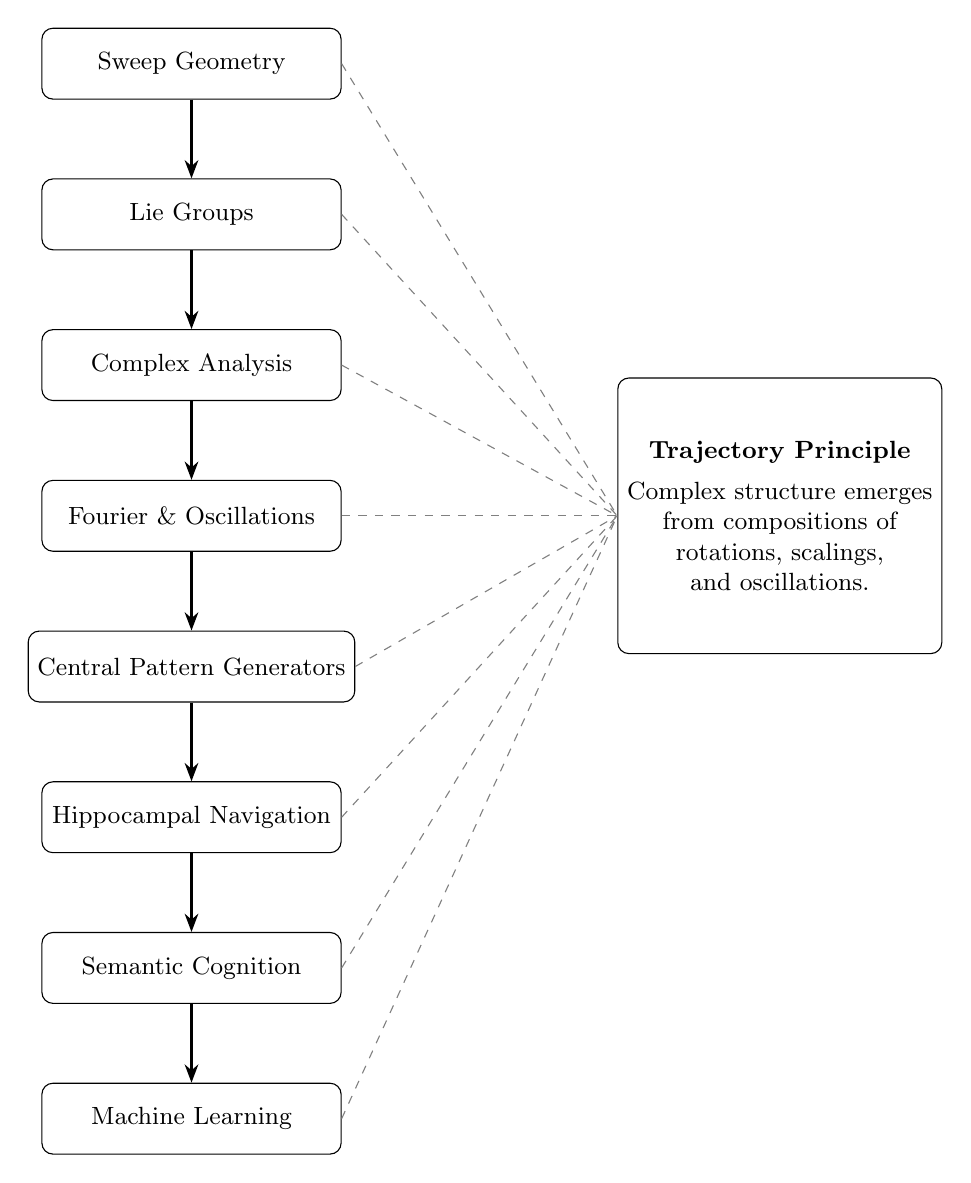
\begin{tikzpicture}[
  level/.style={rectangle,draw,rounded corners,minimum width=3.8cm,
                minimum height=0.9cm,align=center,font=\small},
  arrow/.style={-{Stealth},thick}]

\node[level] (geo) {Sweep Geometry};
\node[level,below=1.0cm of geo] (lie) {Lie Groups};
\node[level,below=1.0cm of lie] (complex) {Complex Analysis};
\node[level,below=1.0cm of complex] (fourier) {Fourier \& Oscillations};
\node[level,below=1.0cm of fourier] (cpg) {Central Pattern Generators};
\node[level,below=1.0cm of cpg] (hippo) {Hippocampal Navigation};
\node[level,below=1.0cm of hippo] (semantic) {Semantic Cognition};
\node[level,below=1.0cm of semantic] (ml) {Machine Learning};

\draw[arrow] (geo)--(lie);
\draw[arrow] (lie)--(complex);
\draw[arrow] (complex)--(fourier);
\draw[arrow] (fourier)--(cpg);
\draw[arrow] (cpg)--(hippo);
\draw[arrow] (hippo)--(semantic);
\draw[arrow] (semantic)--(ml);

\node[right=3.5cm of fourier,align=center,draw,rounded corners,
      minimum width=3.6cm,minimum height=3.5cm,font=\small] (principle)
{\textbf{Trajectory Principle}\\[4pt]
Complex structure emerges\\
from compositions of\\
rotations, scalings,\\
and oscillations.};

\foreach \n in {geo,lie,complex,fourier,cpg,hippo,semantic,ml}
  \draw[dashed,gray] (\n.east) -- (principle.west);
\end{tikzpicture}
\caption{The trajectory stack. Each field independently discovers that complex structure
emerges from compositions of simple geometric transformations. The dashed arrows
indicate that all levels instantiate the same underlying trajectory principle.}
\end{figure}

The universality of the model follows from three classical results taken together.
By the polar decomposition theorem, any linear transformation can be expressed as a
composition of rotation and scaling. By the universal approximation theorem for neural
networks, any continuous function can be approximated by a composition of linear
transformations and nonlinear activations. By the completeness of the Fourier basis,
any square-integrable function can be expressed as a superposition of oscillatory
components, each of which is a rotation in the complex plane. Together these results
imply that any smooth map between manifolds can be approximated to arbitrary precision
by compositions of primitive rotations and scalings. The generating primitives are
universal.

\begin{figure}[h]
\centering
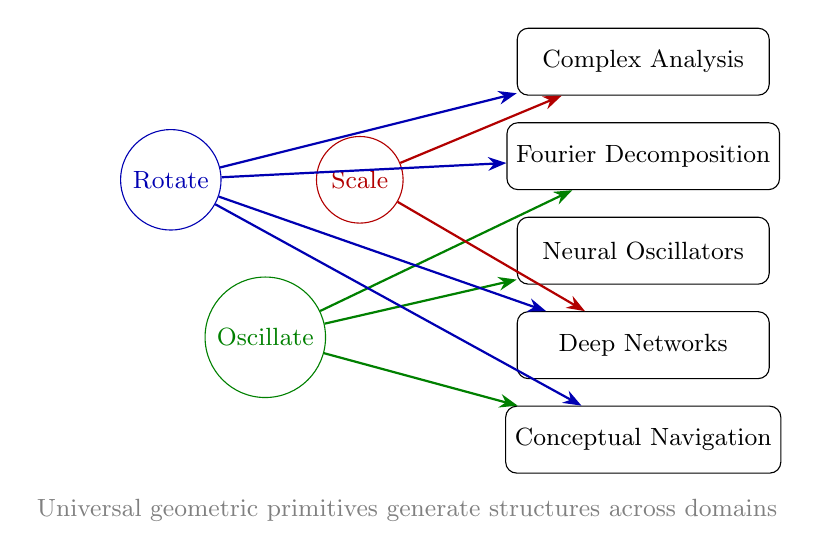
\begin{tikzpicture}[
  op/.style={circle,draw,minimum size=1.1cm,align=center,font=\small},
  box/.style={rectangle,draw,rounded corners,minimum width=3.2cm,
              minimum height=0.85cm,align=center,font=\small},
  arrow/.style={-{Stealth},thick}]

\node[op,blue!70!black] (rot) at (0,0) {Rotate};
\node[op,red!70!black] (scale) at (2.4,0) {Scale};
\node[op,green!50!black] (osc) at (1.2,-2) {Oscillate};

\node[box] (complex) at (6,1.5) {Complex Analysis};
\node[box] (fourier) at (6,0.3) {Fourier Decomposition};
\node[box] (cpg) at (6,-0.9) {Neural Oscillators};
\node[box] (ml) at (6,-2.1) {Deep Networks};
\node[box] (cog) at (6,-3.3) {Conceptual Navigation};

\draw[arrow,blue!70!black] (rot) -- (complex);
\draw[arrow,red!70!black] (scale) -- (complex);
\draw[arrow,blue!70!black] (rot) -- (fourier);
\draw[arrow,green!50!black] (osc) -- (fourier);
\draw[arrow,green!50!black] (osc) -- (cpg);
\draw[arrow,blue!70!black] (rot) -- (ml);
\draw[arrow,red!70!black] (scale) -- (ml);
\draw[arrow,green!50!black] (osc) -- (cog);
\draw[arrow,blue!70!black] (rot) -- (cog);

\node[font=\small,gray] at (3,-4.2)
  {Universal geometric primitives generate structures across domains};
\end{tikzpicture}
\caption{Rotation, scaling, and oscillation function as universal operators generating
complex structures in mathematics, neural systems, and cognition. Each field draws on
a different subset of the three primitives; together they cover all domains discussed
in this essay.}
\end{figure}

A further unification comes from considering the role of entropy in constraining
trajectories. In the RSVP framework developed elsewhere, a scalar entropy field $S$
regulates the behavior of a scalar field $\Phi$ and a vector field $\mathbf{v}$, where
$\Phi$ corresponds to amplitude (scaling) and $\mathbf{v}$ to directional flow
(rotation). The entropy field prevents runaway amplification and constrains the set of
achievable trajectories to a thermodynamically stable manifold. In neural terms this
corresponds to the metabolic and homeostatic limitations of the nervous system; in
computational terms, to regularization conditions imposed during learning. In all cases,
entropy provides a thermodynamic regulator that shapes the geometry of the trajectory
space, determining which paths are stable and which decay.

This unified model does not reduce all cognitive processes to a single mechanism.
Different systems implement the trajectory-generation principle with different geometries
of state space, different transformation groups, and different regulatory constraints.
What the model provides is a common mathematical language for describing all of them.


%%% ─────────────────────────────────────────────────────
\section{Category Theory and the Composition of Transformations}
%%% ─────────────────────────────────────────────────────

If trajectories are the fundamental units of structure, then composition becomes the
fundamental operation. Category theory provides a formal language for describing such
compositional systems.

A category consists of objects and morphisms between them. Morphisms represent
transformations, and the central rule of category theory is that morphisms can be
composed:

\begin{equation}
f : A \to B, \quad g : B \to C
\quad \Rightarrow \quad
g \circ f : A \to C.
\end{equation}

The significance of this structure is that objects are defined not by their internal
composition but by the transformations that connect them to other objects. A morphism
corresponds to a path through transformation space. Composing morphisms corresponds to
chaining trajectories. The identity morphism corresponds to remaining stationary in the
manifold.

Higher category theory extends this framework by allowing morphisms between morphisms,
capturing the relationships among transformations themselves. In such systems, structure
emerges from the network of possible trajectories rather than from the intrinsic nature
of the objects involved. A functor is a structure-preserving map between categories: it
carries objects to objects and morphisms to morphisms, preserving composition. In the
essay's terms, a functor is a transformation of trajectory spaces that respects the
compositional structure.

This categorical perspective illuminates many of the connections drawn in earlier
sections. The relationship between CPG dynamics and hippocampal navigation, for instance,
can be understood as a functor that carries phase-space trajectories of oscillatory
circuits to trajectories through spatial or conceptual manifolds, preserving the
compositional structure of the trajectory algebra. The relationship between image
manifolds and semantic manifolds can be understood similarly. In each case, the relevant
mathematical object is not the spaces themselves but the morphisms between them---the
transformations that carry structure from one domain to another.

Category theory therefore provides a natural mathematical language for the generative
view of structure advanced throughout this essay. Objects become nodes in a web of
transformations, and meaning arises from the ways in which those transformations compose.
This is the precise mathematical form of the essay's central thesis: it is not what
things are that matters but how they transform.


%%% ─────────────────────────────────────────────────────
\section{Evolutionary Origins of Trajectory-Based Cognition}
%%% ─────────────────────────────────────────────────────

The trajectory model of cognition is not merely a mathematical abstraction. It reflects
the evolutionary history of nervous systems.

Early nervous systems evolved to coordinate movement. Locomotion requires integrating
sensory information, predicting environmental changes, and adjusting motor commands in
real time. These tasks are inherently dynamical: they cannot be performed by a system
that merely retrieves static stored representations.

\begin{figure}[h]
\centering
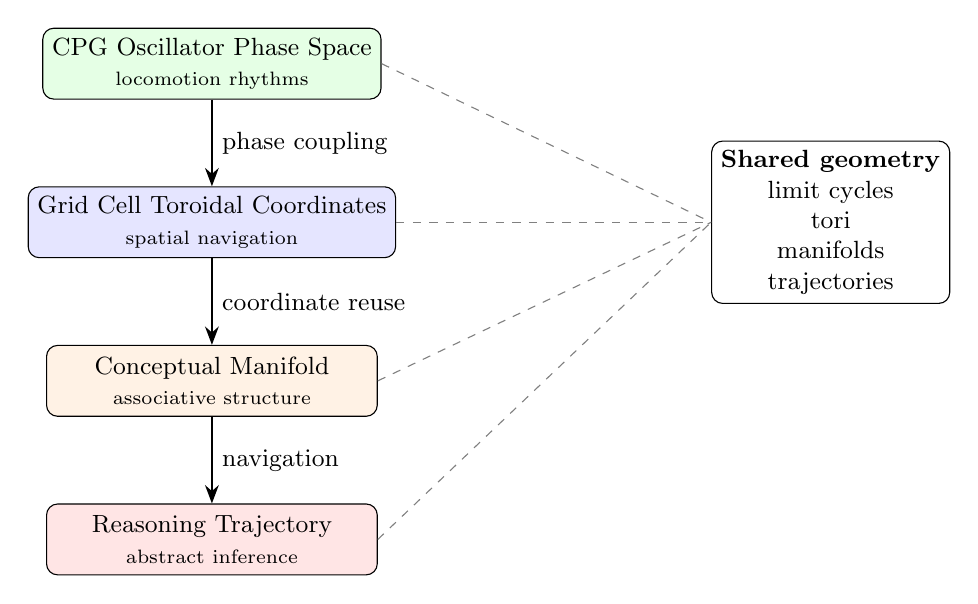
\begin{tikzpicture}[
  level/.style={rectangle,draw,rounded corners,minimum width=4.2cm,
                minimum height=0.9cm,align=center,font=\small},
  arrow/.style={-{Stealth},thick}]

\node[level,fill=green!10] (cpg)
  {CPG Oscillator Phase Space\\{\scriptsize locomotion rhythms}};
\node[level,fill=blue!10,below=1.1cm of cpg] (grid)
  {Grid Cell Toroidal Coordinates\\{\scriptsize spatial navigation}};
\node[level,fill=orange!10,below=1.1cm of grid] (concept)
  {Conceptual Manifold\\{\scriptsize associative structure}};
\node[level,fill=red!10,below=1.1cm of concept] (reason)
  {Reasoning Trajectory\\{\scriptsize abstract inference}};

\draw[arrow] (cpg)--node[right,font=\small]{phase coupling}(grid);
\draw[arrow] (grid)--node[right,font=\small]{coordinate reuse}(concept);
\draw[arrow] (concept)--node[right,font=\small]{navigation}(reason);

\node[right=4cm of grid,align=center,draw,rounded corners,font=\small,
      minimum width=2.8cm] (geometry)
{\textbf{Shared geometry}\\limit cycles\\tori\\manifolds\\trajectories};

\foreach \n in {cpg,grid,concept,reason}
  \draw[dashed,gray] (\n.east) -- (geometry.west);
\end{tikzpicture}
\caption{The cognitive phase-space hierarchy. The same phase-space geometry appears
across evolutionary timescales and levels of organization: motor oscillators generate
toroidal dynamics, grid cells reuse that structure for spatial coordinates, conceptual
spaces inherit the same manifold geometry, and reasoning corresponds to trajectories
through that manifold.}
\end{figure}

Central pattern generators provided the earliest neural mechanisms for producing
coordinated motion. The oscillatory dynamics of these circuits created stable trajectories
in phase space that could be modulated by sensory input. As nervous systems became more
complex, the same dynamical mechanisms were recruited for new purposes. Spatial
navigation reused locomotor oscillators to track position. Conceptual reasoning reused
spatial navigation circuits to traverse abstract spaces of meaning. This hypothesis of
neural reuse has gained substantial empirical support: the same areas of the hippocampal
formation that process spatial coordinates also process abstract conceptual relationships,
and the same grid-cell periodicity that tiles physical space also tiles conceptual space.

From an evolutionary perspective, abstract cognition did not arise by inventing entirely
new mechanisms. Instead, existing trajectory-generating systems were repurposed for
increasingly abstract forms of navigation. The abstract structures of semantic memory,
planning, and inference inherit their geometry from the oscillatory and navigational
dynamics of far more ancient motor systems. The mind therefore retains the dynamical
architecture of its origins. Even the most abstract reasoning processes can be understood
as descendants of the mechanisms that once coordinated movement through physical
environments. The philosopher's claim that thought is inner speech has an older
predecessor: thought is inner locomotion, the navigation of a terrain made internal.


%%% ─────────────────────────────────────────────────────
\section{Empirical Predictions}
%%% ─────────────────────────────────────────────────────

The trajectory framework developed in this essay generates several testable predictions.
Stating them explicitly distinguishes the framework from a purely philosophical thesis
and opens it to scientific evaluation.

First, neural population activity during conceptual reasoning should exhibit rotational
dynamics similar to those observed in motor cortex and hippocampal navigation circuits.
Dimensionality reduction methods such as jPCA should reveal phase-space rotations
corresponding to conceptual transitions. Rotational dynamics have already been observed
in motor cortex during movement preparation; if the trajectory model is correct,
analogous rotations should appear in areas associated with semantic processing and
abstract reasoning, and their phase structure should correspond to the semantic distance
between concepts being traversed.

Second, learned representations in artificial neural networks should organize
transformations along low-dimensional manifolds whose generators correspond to
interpretable geometric operations such as rotation, scaling, or translation.
Specifically, the Fisher information metric on the parameter manifold of a well-trained
network should exhibit a low effective dimensionality, reflecting the fact that the
network has found a compact set of generators for its input-output mapping.

Third, perturbations of oscillatory phase relationships in neural circuits should disrupt
both motor coordination and conceptual navigation, reflecting their shared dynamical
substrate. Targeted disruption of hippocampal theta oscillations, for instance, should
impair not only spatial navigation performance but also the speed and accuracy of
semantic inference on structured conceptual spaces, particularly for inferences that
require traversing multiple attractor basins in sequence.

Fourth, behavioral measures of reasoning should exhibit temporal characteristics
consistent with trajectory traversal, including inertia, gradient-following dynamics,
and attractor basin transitions. Specifically, the time required to make a semantic
inference should increase with the conceptual distance between the starting concept and
the target concept, measured along the geodesic of the semantic manifold, not simply as
a function of the number of associative steps between them as counted in a static network.

Fifth, subjects trained in environments that impose oscillatory structure---rhythmic
locomotion, music, breathing exercises with controlled phase---should show enhanced
performance on conceptual navigation tasks that require traversal of multiple attractor
basins, if the hypothesis is correct that the shared dynamical substrate can be
recruited across domains.

Testing these predictions would provide empirical support for the hypothesis that
cognition is fundamentally a process of navigating representational manifolds, and would
distinguish the trajectory model from the storage-retrieval model with which it competes.


%%% ─────────────────────────────────────────────────────
\section{The Trajectory Ladder of Dimension and Cognition}
%%% ─────────────────────────────────────────────────────

The argument of this essay can be compressed into a single diagram. Each level in the
following ladder arises from the trajectory of the level below it, and the same
generative logic that carries a point to a line carries an oscillatory phase space to a
conceptual manifold.

\begin{figure}[h]
\centering
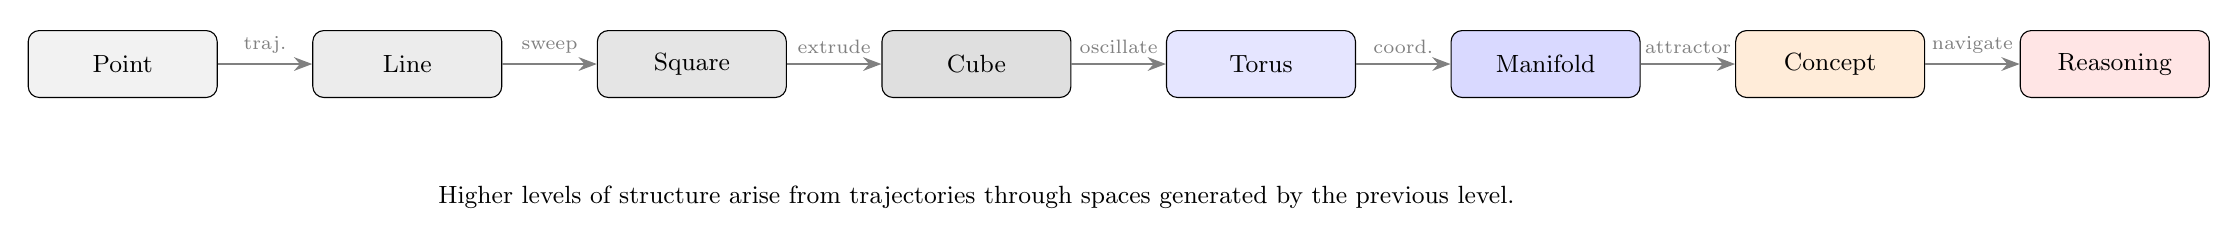
\begin{tikzpicture}[
  level/.style={rectangle,draw,rounded corners,minimum width=2.4cm,
                minimum height=0.85cm,align=center,font=\small},
  arrow/.style={-{Stealth},thick,gray}]

\node[level,fill=gray!10] (point) {Point};
\node[level,fill=gray!15,right=1.2cm of point] (line) {Line};
\node[level,fill=gray!20,right=1.2cm of line] (square) {Square};
\node[level,fill=gray!25,right=1.2cm of square] (cube) {Cube};
\node[level,fill=blue!10,right=1.2cm of cube] (torus) {Torus};
\node[level,fill=blue!15,right=1.2cm of torus] (mfld) {Manifold};
\node[level,fill=orange!15,right=1.2cm of mfld] (concept) {Concept};
\node[level,fill=red!10,right=1.2cm of concept] (thought) {Reasoning};

\draw[arrow] (point)--node[above,font=\scriptsize]{traj.}(line);
\draw[arrow] (line)--node[above,font=\scriptsize]{sweep}(square);
\draw[arrow] (square)--node[above,font=\scriptsize]{extrude}(cube);
\draw[arrow] (cube)--node[above,font=\scriptsize]{oscillate}(torus);
\draw[arrow] (torus)--node[above,font=\scriptsize]{coord.}(mfld);
\draw[arrow] (mfld)--node[above,font=\scriptsize]{attractor}(concept);
\draw[arrow] (concept)--node[above,font=\scriptsize]{navigate}(thought);

\node[below=1.0cm of cube,align=center,font=\small]
{Higher levels of structure arise from trajectories through spaces generated
by the previous level.};
\end{tikzpicture}
\caption{The trajectory ladder of dimension and cognition. Geometric objects arise
from swept trajectories of lower-dimensional predecessors; conceptual and cognitive
structures arise from trajectories through representational manifolds generated by
neural dynamics. Each step adds a new independent direction of generative freedom.}
\end{figure}

The first four steps---point, line, square, cube---correspond to the sweep geometry
of the second section. The transition from cube to torus corresponds to the move from
static polyhedra to oscillatory dynamical systems, where two independent phase variables
generate a toroidal phase space. The transition from torus to manifold corresponds to
the move from simple periodic dynamics to the rich, curved representational geometry
of hippocampal and cortical systems. The transition from manifold to concept corresponds
to the formation of attractor basins within that manifold. And the transition from
concept to reasoning corresponds to navigation through those basins, following
trajectories shaped by contextual gradients and associative structure.

At each step, the entity at the new level is not a new kind of thing in a categorically
different realm; it is the record of a trajectory through the space generated by the
previous level. This is the deepest form of the essay's claim, and the diagram makes
it visual. Structure is generated, not stored. Dimension is not intrinsic but earned
through motion. And cognition, at its most abstract, is geometry at its most dynamic.


%%% ─────────────────────────────────────────────────────
\section{Philosophical Consequences: From Storage to Generation}
%%% ─────────────────────────────────────────────────────

The geometric model developed in the preceding sections has philosophical consequences
that reach beyond the specific scientific domains it addresses. These consequences
concern the nature of representation, the structure of knowledge, and the relationship
between cognition and world.

The prevailing model of mental representation is what might be called the
storage-retrieval model. Representations are encoded, stored in memory, and retrieved
when needed. Knowledge is a warehouse. Reasoning is the manipulation of stored
representations according to rules. The mind is analogous to a library: it contains
information, organized for access.

The trajectory model proposed in this essay is fundamentally at odds with this picture.
What the storage-retrieval model calls a representation is not a stored entity but a
reproducible trajectory. A memory is not a pattern inscribed in synaptic weights but a
trajectory the system can reconstruct from partial initial conditions. A concept is not
a node with a fixed content but an attractor basin that shapes the trajectories of
activation that pass through it. Knowledge is not a set of stored facts but a
configuration of the system's trajectory space---a set of paths the system can reliably
follow through its representational manifold.

\begin{figure}[h]
\centering
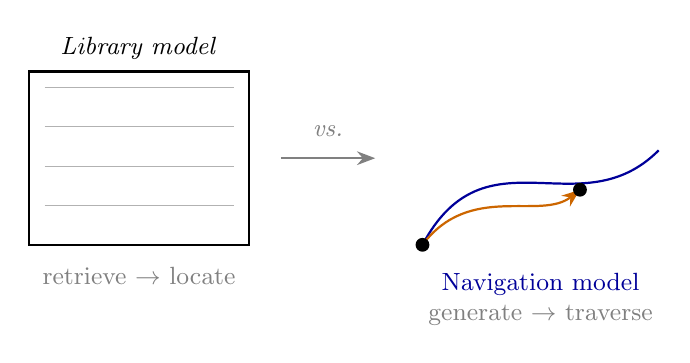
\begin{tikzpicture}[scale=1.0]
% Library box
\draw[thick] (0,0) rectangle (2.8,2.2);
\foreach \y in {0.5,1.0,1.5,2.0}
  \draw[gray!60] (0.2,\y)--(2.6,\y);
\node[font=\small] at (1.4,2.5) {\textit{Library model}};
\node[font=\small,gray] at (1.4,-0.4) {retrieve $\to$ locate};

% Arrow
\draw[-{Stealth},thick,gray] (3.2,1.1) -- (4.4,1.1);
\node[font=\small,gray] at (3.8,1.45) {\textit{vs.}};

% Navigation
\begin{scope}[xshift=5cm]
\draw[thick,blue!60!black]
  (0,0) .. controls (0.8,1.5) and (2.0,0.2) .. (3,1.2);
\draw[-{Stealth},orange!80!black,thick]
  (0,0) .. controls (0.6,0.8) and (1.5,0.3) .. (2,0.7);
\fill (0,0) circle (2.5pt);
\fill (2,0.7) circle (2.5pt);
\node[font=\small,blue!60!black] at (1.5,-0.5) {Navigation model};
\node[font=\small,gray] at (1.5,-0.9) {generate $\to$ traverse};
\end{scope}
\end{tikzpicture}
\caption{Knowledge as storage versus knowledge as navigation. The library model treats
cognition as retrieval of fixed items from fixed locations. The navigation model treats
cognition as the generation of trajectories through a structured terrain. The same
points appear in both views, but only the navigation model captures the dynamical
process by which they are produced.}
\end{figure}

The trajectory model aligns with, and provides mathematical precision for, the tradition
of embodied cognition in philosophy and cognitive science. Embodied cognition holds that
cognition is not the manipulation of abstract symbols inside an isolated brain but a
process constitutively involving the body and its environment. The hippocampal findings
reviewed in earlier sections provide direct neural evidence: the spatial representations
constructed by place and grid cells are not stored in the cells but generated through
movement, through the path integration of self-motion signals over time. The map is made,
not found.

Hiott's way-making account extends this insight explicitly to semantic cognition.
Understanding a concept is not accessing a stored definition; it is traversing a region
of conceptual space, navigating among associated ideas, following the gradient of an
attractor basin to its center. The meaning is the trajectory, not the destination.

A further philosophical implication concerns the relationship between individual and
social cognition. Language provides a set of external landmarks in conceptual space---
words and sentences that function as attractors, orienting the trajectories of individual
cognitive systems toward socially coordinated destinations. The meaning of a word is not
a private representation stored in each speaker's mind but a convergence of trajectories
in a shared conceptual manifold, maintained through the ongoing practice of using
language together.

If structures arise from trajectories rather than from storage, then knowledge, meaning,
perception, and reasoning all need to be reconceived as processes of navigation through
structured spaces rather than as operations on fixed representations. The mind is not a
library but a vehicle, and its knowledge is not stored in it but enacted by it.


%%% ─────────────────────────────────────────────────────
\section{Conclusion: Movement as the Generative Principle}
%%% ─────────────────────────────────────────────────────

This essay has traced a single geometric insight across thirteen domains. The insight is
this: simple transformations---scaling, rotation, and oscillation---compose to generate
complex structure, and what appears as a stable object in mathematics, neuroscience, or
computation is, at a deeper level, the stabilized record of a trajectory produced by
chaining such transformations.

In classical geometry, dimension is the number of independent directions of motion
required to generate an object. In Lie theory, global transformations are generated from
infinitesimal ones; the Lie algebra provides the minimal vocabulary of motions from
which the entire transformation group is navigated. In complex analysis, holomorphic
functions are locally amplitwists---simultaneous rotations and scalings---and complicated
conformal mappings arise from composing many such local operations across a domain.
In signal processing and machine learning, oscillatory primitives generate universal
approximations to arbitrary functions. In biological motor systems, central pattern
generators implement oscillatory rotation in phase space. In the hippocampal formation,
spatial and conceptual representations are constructed through path integration of
movement signals. In semantic cognition, concepts are attractor basins and reasoning is
navigation. In transformation spaces and latent representations, adjustable parameters
correspond to directions in a geometrically structured space. In information geometry,
learning is geodesic descent on the statistical manifold. In category theory, composition
of morphisms is the fundamental operation and objects derive meaning from their
transformation relations.

Across all these domains, the pattern is the same. Simple primitives compose. The
composition generates structure. The structure is a trajectory, not a location.
The system is a vehicle, not a warehouse.

The evolutionary picture reinforces this conclusion: the nervous system did not invent
abstract cognition from nothing. It repurposed the trajectory-generating machinery of
motor systems for increasingly abstract navigation. The same oscillatory circuits that
once guided a worm through a gradient of nutrients now, in elaborated form, navigate
the conceptual gradients of a mathematical proof.

This view demands a revision of the metaphors through which cognition is usually
imagined. The library metaphor should give way to the navigation metaphor: knowledge as
a structured terrain, thinking as movement through it. The computer metaphor should give
way to the dynamical systems metaphor: the brain as a trajectory generator, producing
behavior by navigating a high-dimensional phase space shaped by the geometry of the
organism's embodied history. These are not merely aesthetic choices. They determine what
scientific questions are asked, what experiments are designed, and what models are built.

Scaling, rotation, and oscillation are not merely tools of mathematics; they are the
generative principles by which the universe, and the minds that inhabit it, produce
structure from motion.

The line is a moving point. The cube is a moving square. The concept is a moving
activation. The thought is a moving mind.

\bigskip
\noindent\rule{\textwidth}{0.4pt}
\bigskip


%%% ─────────────────────────────────────────────────────
\appendix
\section{Mathematical Appendix: Amplitwist as a Conformal Polar Decomposition}
%%% ─────────────────────────────────────────────────────

This appendix formalizes the geometric claim used throughout the essay: the derivative
of a holomorphic function acts locally as a rotation together with a uniform scaling,
and this local amplitwist is a special two-dimensional conformal case of the general
polar decomposition for invertible linear maps.

\subsection{Complex differentiation as local linearization}

Let $f:\mathbb{C}\to\mathbb{C}$ be complex differentiable at $z_0$. By definition,
there exists a complex number $f'(z_0)$ such that

\begin{equation}
\lim_{\varepsilon\to 0}
\frac{f(z_0+\varepsilon)-f(z_0)-f'(z_0)\varepsilon}{\varepsilon}=0.
\end{equation}

Equivalently, there exists a remainder term $r(\varepsilon)$ with

\begin{equation}
f(z_0+\varepsilon)=f(z_0)+f'(z_0)\varepsilon+r(\varepsilon),
\qquad
\frac{r(\varepsilon)}{\varepsilon}\to 0
\text{ as }
\varepsilon\to 0.
\label{eq:appendix_linearization}
\end{equation}

\begin{theorem}[Local amplitwist decomposition]
Let $f:\mathbb{C}\to\mathbb{C}$ be holomorphic at $z_0$ with $f'(z_0)\neq 0$.
Then there exist unique numbers $\rho>0$ and $\theta\in\mathbb{R}$ such that

\begin{equation}
f'(z_0)=\rho e^{i\theta},
\end{equation}

and the first-order action of $f$ near $z_0$ is a composition of a uniform scaling
by $\rho$ and a rotation by angle $\theta$.
\end{theorem}

\begin{proof}
Write the derivative in polar form,
\[
f'(z_0)=\rho e^{i\theta}, \quad \rho=|f'(z_0)|>0, \quad \theta=\arg f'(z_0).
\]
Substituting into \eqref{eq:appendix_linearization} gives
\[
f(z_0+\varepsilon)=f(z_0)+\rho e^{i\theta}\varepsilon+r(\varepsilon).
\]
Multiplication by $e^{i\theta}$ rotates every vector in the complex plane by angle
$\theta$, while multiplication by $\rho$ scales every vector length by $\rho$.
Since $r(\varepsilon)=o(\varepsilon)$, the remainder is negligible for sufficiently
small $\varepsilon$. Hence the local action of $f$ is, to first order, exactly a
rotation followed by a uniform scaling.
\end{proof}

\begin{corollary}[Conformality]
If $f$ is holomorphic at $z_0$ and $f'(z_0)\neq 0$, then $f$ preserves oriented
angles at $z_0$.
\end{corollary}

\begin{proof}
A rotation preserves all angles, and a uniform scaling preserves all angles.
Their composition therefore preserves all angles.
\end{proof}

\subsection{Real Jacobian form and the Cauchy--Riemann constraint}

Write $z=x+iy$ and $f(z)=u(x,y)+iv(x,y)$.
If $f$ is holomorphic, the Cauchy--Riemann equations hold:

\begin{equation}
u_x=v_y, \qquad u_y=-v_x.
\end{equation}

Hence the real Jacobian takes the special form

\begin{equation}
J_f(z_0)=
\begin{pmatrix}
a & -b \\
b & a
\end{pmatrix},
\qquad
a=\Re f'(z_0),
\qquad
b=\Im f'(z_0).
\label{eq:appendix_cr_matrix}
\end{equation}

\begin{proposition}[Similarity form of the holomorphic Jacobian]
If $f$ is holomorphic at $z_0$ and $f'(z_0)\neq 0$, then
\[
J_f(z_0)^T J_f(z_0)=|f'(z_0)|^2 I.
\]
Therefore $J_f(z_0)$ is a similarity transformation: it preserves angles and scales
all directions equally.
\end{proposition}

\begin{proof}
From \eqref{eq:appendix_cr_matrix},
\[
J_f(z_0)^T J_f(z_0)
=
\begin{pmatrix}a & b\\-b & a\end{pmatrix}
\begin{pmatrix}a & -b\\b & a\end{pmatrix}
=
(a^2+b^2)I
=
|f'(z_0)|^2 I.
\qedhere
\]
\end{proof}

\subsection{General polar decomposition}

\begin{theorem}[Polar decomposition]
Let $A\in GL(n,\mathbb{R})$. Then there exist unique matrices
$R\in O(n)$ and $S$ symmetric positive definite such that

\begin{equation}
A=RS,
\qquad
S=(A^T A)^{1/2},
\qquad
R=A S^{-1}.
\end{equation}
\end{theorem}

\begin{proof}
Since $A$ is invertible, $A^T A$ is symmetric positive definite with unique positive
square root $S=(A^T A)^{1/2}$. Define $R=A S^{-1}$. Then
\[
R^T R = S^{-T}A^T A S^{-1} = S^{-1}S^2 S^{-1} = I,
\]
so $R$ is orthogonal. Uniqueness follows from the uniqueness of the positive square
root of $A^T A$.
\end{proof}

\begin{corollary}[Amplitwist as conformal polar decomposition]
If $A$ is the real Jacobian of a holomorphic map at a point, then its polar factor
$S=\rho I$ for some $\rho>0$, and its orthogonal factor $R$ is a planar rotation. Thus

\begin{equation}
A
=
\underbrace{
\begin{pmatrix}
\cos\theta & -\sin\theta\\
\sin\theta & \cos\theta
\end{pmatrix}}_{R}
\underbrace{
\begin{pmatrix}
\rho & 0\\
0 & \rho
\end{pmatrix}}_{S}.
\end{equation}

So the amplitwist decomposition is exactly the isotropic, conformal, two-dimensional
special case of polar decomposition.
\end{corollary}

\begin{proof}
From the proposition above, $A^T A=\rho^2 I$ for $\rho=|f'(z_0)|$.
Therefore $S=(A^T A)^{1/2}=\rho I$.
The orthogonal factor $R=A S^{-1}$ is then an orientation-preserving orthogonal matrix
in two dimensions, hence a planar rotation.
\end{proof}

\begin{figure}[h]
\centering
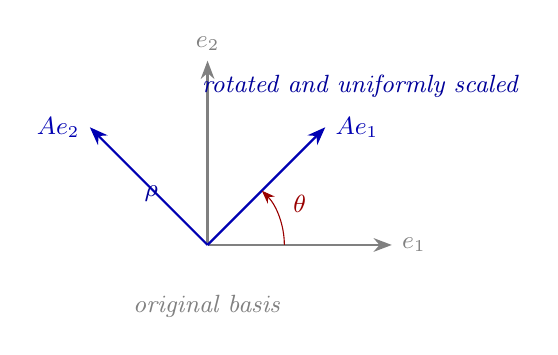
\begin{tikzpicture}[scale=1.3]
% Original basis
\draw[-{Stealth},gray,thick] (0,0) -- (1.8,0) node[right]{\small$e_1$};
\draw[-{Stealth},gray,thick] (0,0) -- (0,1.8) node[above]{\small$e_2$};

% Transformed basis
\draw[blue!70!black,thick,-{Stealth}] (0,0) -- (1.15,1.15)
  node[right,font=\small]{$Ae_1$};
\draw[blue!70!black,thick,-{Stealth}] (0,0) -- (-1.15,1.15)
  node[left,font=\small]{$Ae_2$};

% Angle arc
\draw[-{Stealth},red!60!black] (0.75,0) arc (0:45:0.75);
\node[red!60!black,font=\small] at (0.9,0.4) {$\theta$};

% Rho label
\node[blue!60!black,font=\small] at (-0.55,0.5) {$\rho$};

\node[font=\small,gray] at (0,-0.6) {\textit{original basis}};
\node[blue!60!black,font=\small] at (1.5,1.55) {\textit{rotated and uniformly scaled}};
\end{tikzpicture}
\caption{Local amplitwist action on the standard basis. A holomorphic derivative sends
the orthogonal basis $\{e_1,e_2\}$ to another orthogonal basis, rotated by $\theta$ and
uniformly scaled by $\rho$. No shear or anisotropic stretching occurs; this is the
distinctive property of conformal maps.}
\end{figure}

\subsection{Interpretive summary}

The general polar decomposition says that every invertible linear map can be written
as an orthogonal part and a positive stretching part. The holomorphic case is special
because the stretching part is isotropic rather than anisotropic: every direction is
scaled equally. The derivative of a holomorphic map does not merely stretch and rotate;
it stretches uniformly and rotates, which is why it preserves angles.

For a general real linear map $A$, the symmetric factor $S$ may scale different
directions by different amounts, introducing anisotropic stretching equivalent to a
shear after composition with $R$. This is precisely what fails in the non-holomorphic
case: the violation of the Cauchy--Riemann equations is equivalent to the introduction
of anisotropy into the polar factor $S$. Conformality and isotropic scaling are
equivalent conditions, both captured by the requirement that $A^T A = \rho^2 I$.

This is the mathematical sense in which the amplitwist acts as a prototype for the
broader operator framework of the essay. Whenever a system can be modeled locally by
operators of the form $\mathrm{rotation}\times\mathrm{scaling}$, it inherits the same
basic geometry as the derivative of a holomorphic map, with all the properties---
conformality, universality of composition, and the compact parameterization by just two
real numbers $\rho$ and $\theta$---that follow from it.


%%% ─────────────────────────────────────────────────────
\section*{References}
%%% ─────────────────────────────────────────────────────

\begin{description}[leftmargin=2em, itemsep=0.5em]

\item Amari, S. (2016). \textit{Information Geometry and Its Applications}. Springer.

\item Gärdenfors, P. (2000). \textit{Conceptual Spaces: The Geometry of Thought}.
MIT Press.

\item Hiott, A. (2025). Radical embodied relation at any scale, from remembering
to navigating. \textit{Topoi}. Advance online publication.
\href{https://doi.org/10.1007/s11245-025-10256-7}{https://doi.org/10.1007/s11245-025-10256-7}

\item Hopfield, J. J. (1982). Neural networks and physical systems with emergent
collective computational abilities. \textit{Proceedings of the National Academy of
Sciences}, 79(8), 2554--2558.

\item Kuramoto, Y. (1984). \textit{Chemical Oscillations, Waves, and Turbulence}.
Springer.

\item Mac Lane, S. (1998). \textit{Categories for the Working Mathematician} (2nd ed.).
Springer.

\item Moser, E. I., Kropff, E., \& Moser, M.-B. (2008). Place cells, grid cells, and
the brain's spatial representation system. \textit{Annual Review of Neuroscience},
31, 69--89.

\item Needham, T. (1997). \textit{Visual Complex Analysis}. Oxford University Press.

\item O'Keefe, J., \& Nadel, L. (1978). \textit{The Hippocampus as a Cognitive Map}.
Oxford University Press.

\item Strogatz, S. H. (2014). \textit{Nonlinear Dynamics and Chaos: With Applications
to Physics, Biology, Chemistry, and Engineering} (2nd ed.). Westview Press.

\item Tolman, E. C. (1948). Cognitive maps in rats and men. \textit{Psychological
Review}, 55(4), 189--208.

\item van Vreeswijk, C., \& Sompolinsky, H. (1996). Chaos in neuronal networks with
balanced excitatory and inhibitory activity. \textit{Science}, 274(5293), 1724--1726.

\item Yartsev, M. M., \& Ulanovsky, N. (2013). Representation of three-dimensional
space in the hippocampus of flying bats. \textit{Science}, 340(6130), 367--372.

\end{description}

\end{document}
